%!TEX root = handout.tex

\newpage
\section{Quality control}
\label{sec:qc}

\subsection{Introduction}

In this chapter, we will build on an existing workflow with OpenMS / KNIME to add some quality control (QC). We will utilize the qcML tools in OpenMS to create a file with which we can collect different measures of quality to the mass spectrometry runs themselves and the applied analysis. The file also serves the means of visually reporting on the collected quality measures and later storage along the other analysis result files.
We will, step-by-step, extend the label-free quantitation workflow from section \ref{sec:lfq} with QC functions and thereby enrich each time the report given by the qcML file.
But first, to make sure you get the most of this tutorial section, a little primer on how we handle QC on the technical level. \\

\subsubsection*{QC metrics and qcML}
To assert the quality of a measurement or analysis we use quality metrics. Metrics are describing a certain aspect of the measurement or analysis and can be anything from a single value, over a range of values to a image plot or other summary. Thus, qcML metric representation is divided into QC parameters (QP) and QC attachments (QA) to be able to represent all sorts of metrics on a technical level.\\
A QP may (or may not) have a value which would equal a metric describable with a single value. If the metric is more complex and needs more than just a single value, the QP does not require the single value but rather depends on an attachment of values (QA) for full meaning. Such a QA holds the plot or the range of values in a table-like form. Like this, we can describe any metric by a QP and an optional QA.\\
To assure a consensual meaning of the quality parameters and attachments, we created a controlled vocabulary (CV). Each entry in the CV describes a metric or part/extension thereof. We embed each parameter or attachment with one of these and by doning so, connect a meaning to the QP/QA. Like this, we later know exactly what we collected and the programs can find and connect the right dots for rendering the report or calculating new metrics automatically. You can find the constantly growing controlled vocabulary here:\\ \menu{https://github.com/qcML/qcML-development/blob/master/cv/qc-cv.obo}.\\
Finally, in a qcml file, we split the metrics on a per mass-spectrometry-run base or a set of mass-spectrometry-runs respectively. Each run or set will contain its QP/QA we calculate for it, describing their quality.


\subsection{Building a qcML file per run}
\label{Building a qcML file per run}

As a start, we will build a basic qcML file for each mzML file in the label-free analysis. We are already creating the two necessary analysis files to build a basic qcML file upon each mzML file, a feature file and an identification file. We use the \KNIMENODE{QCCreator} node from \menu{Community Nodes > OpenMS > Utilities} where also all other \KNIMENODE{QC*} nodes will be found. The \KNIMENODE{QCCreator} will create a very basic qcML file in which it will store collected and calculated quality data.

\begin{itemize} 
\item Copy your label-fee quantitation workflow into a new lfq-qc workflow and open it.
\item Place the \KNIMENODE{QCCreator} node after the \KNIMENODE{IDMapper} node. Being inside the \KNIMENODE{ZipLoop}, it will execute for each of the three mzML files the \KNIMENODE{Input} node.
\item Connect the first \KNIMENODE{QCCreator} port to the first \KNIMENODE{ZipLoopStart} outlet port, which will carry the individual mzML files.
\item Connect the last's \KNIMENODE{ID} outlet port (\KNIMENODE{IDFilter} or the \KNIMENODE{ID} metanode) to the second \KNIMENODE{QCCreator} port for the identification file.
\item Finally, connect the \KNIMENODE{IDMapper} outlet to the third \KNIMENODE{QCCreator} port for the feature file.
\end{itemize}

The created qcML files will not have much to show for, basic as they are. So we will extend them with some basic plots.
\begin{itemize}
\item First, we will add an 2D overview image of the given mass spectrometry run as you may know it from \OPENMSTOOL{TOPPView}. Add a the \KNIMENODE{ImageCreator} node from \menu{Community Nodes > OpenMS > Utilities}. Change the \textit{width} and \textit{heigth} parameters to 640x640 as we don't want it to be too big. Connect it the first \KNIMENODE{ZipLoopStart} outlet port, so it will create an image file of the mzML's contained run.
\item Now we have to embed this file into the qcML file, attach it to the right QualityParameter. For this, place a \KNIMENODE{QCEmbedder} node behind the \KNIMENODE{ImageCreator} and connect that to its third inlet port. Its first inlet port connect to the outlet of the \KNIMENODE{QCCalculator} node to pass on the qcML file. Now change the parameter \textit{qp\_att\_acc} to \textit{QC:0000055} which designates the attached image to be of type  \texttt{QC:0000055 - MS experiment heatmap}.
Finally, change the parameter \textit{cv\_acc} to \textit{QC:0000004}, to attach the image to the QualityParameter \texttt{QC:0000004 - MS acquisition result details}.
\item For a reference of which CVs are already defined for qcML, have a look at \\ \menu{https://github.com/qcML/qcML-development/blob/master/cv/qc-cv.obo}.
\end{itemize}

There are two other basic plots which we almost always might want to look at before judging the quality of a mass spectrometry run and its identifications: the \textit{total ion current} (TIC) and the \textit{PSM mass error} (Mass accuracy), which we have available as pre-packaged QC metanodes.
\begin{task}
Import the workflow from \directory{Workflows / QC Metanodes.zip} in KNIME: \menu{File > Import KNIME Workflow...}
\end{task}
\begin{itemize}
\item Copy the \KNIMENODE{Mass accuracy} metanode into the workflow behind the \KNIMENODE{QCEmbedder} node and connect it. The qcML will be passed on and the Mass accuracy plots added. The information needed was already collected by the \KNIMENODE{QCCalculator}.
\item Do the same with the \KNIMENODE{TIC} metanode so that your qcML file will get passed on and enriched on each step. 
\end{itemize}
\begin{figure}[htbp]
  \centering
  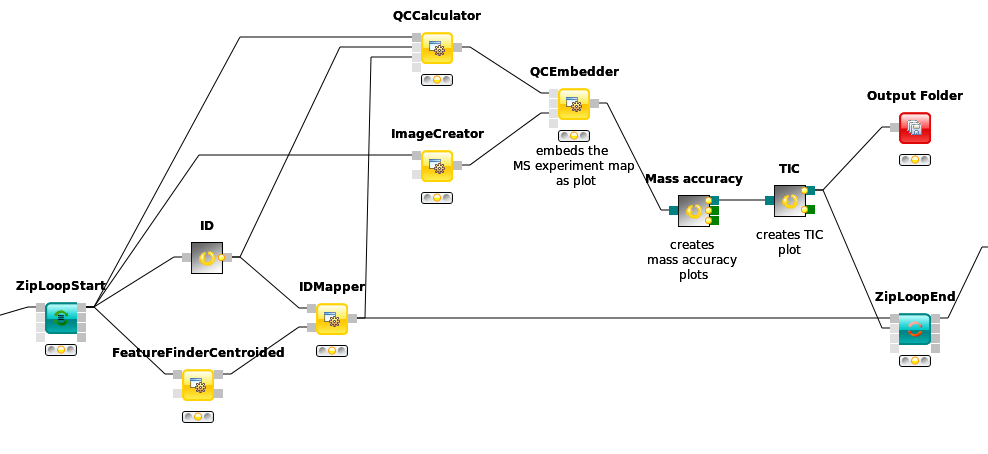
\includegraphics[width=0.85\textwidth]{graphics/qc/qc_basic}
  \caption{Basic QC setup within a LFQ workflow}
  \label{fig:qc_basic}
\end{figure}

\note{To have a peek into what our qcML now looks like for one of the \KNIMENODE{ZipLoop} iterations, we can add an \KNIMENODE{Output Folder} node from \menu{Community Nodes > GenericKnimeNodes > IO} and set its destination paramter to somewhere we want to find our intermediate qcML files in, for example \menu{tmp > qc\_lfq}. If we now connect the last metanode with the \KNIMENODE{Output Folder} and restart the workflow, we can start inspecting the qcML files. Just open them with the browser, and the contained QC parameter will be rendered for you.}


\subsection{Adding brand new QC metrics}
\label{Adding brand new QC metrics}

We can also add brand new QC metrics to our qcML files. Remember the \KNIMENODE{Histogram} you added inside the \KNIMENODE{ZipLoop} during the label-free quantitation section? %TODO reference
 Let's imagine for a moment this was a brand new and utterly important metric and plot for the assessment of your analyses quality. There is an easy way to pick up such new finds along the workflow into your qcMLs. Though the \KNIMENODE{Histogram} node cannot pass its plot to an \textit{image}, we will do with a \KNIMENODE{R View (table)}. 

\begin{itemize}
\item Add an \KNIMENODE{R View (table)} next to the \KNIMENODE{IDTextReader} node and connect them.
\item Edit the \KNIMENODE{R View (table)} by adding the \textit{R Script} according to this:
\end{itemize}
\begin{lstlisting}
#install.packages("ggplot2")
library("ggplot2")
ggplot(knime.in, aes(x=peptide_charge)) + 
 geom_histogram(binwidth=1, origin =-0.5) + 
 scale_x_discrete() + 
 ggtitle("Identified peptides charge histogram") + 
 ylab("Count")
\end{lstlisting}
\begin{itemize}
\item This will create a plot like the \KNIMENODE{Histogram} node on \textit{peptide\_charge} \textbf{and} pass it on as an \textit{image}. 
\item Now add and connect a \KNIMENODE{Image2FilePort} node from \menu{Community Nodes > GenericKnimeNodes > Flow} to the \KNIMENODE{R View (table)}.
\item We can now use a \KNIMENODE{QCEmbedder} node like before to add our new metric plot into the qcML.
\item After looking for an appropriate target in \\ \menu{https://github.com/qcML/qcML-development/blob/master/cv/qc-cv.obo}, we found that we can attach our plot to the \textit{MS identification result details} by setting the parameter \textit{qp\_att\_acc} to \textit{QC:0000025}, as we are plotting the charge histogram of our \textit{identified} peptides.
\item To have the plot later displayed properly, we assign it the parameter \textit{cv\_acc} of \textit{QC:0000051}, a \textit{generic plot}. Also we made sure in the \textit{R Script}, that our plot carries a caption so that we know which is which, if we had more than one new plot.
\item Now we redirect the \KNIMENODE{QCEmbedder}s output to the \KNIMENODE{Output Folder} from before and can have a look at how our qcML is coming along after restarting the workflow.
\end{itemize}

\begin{figure}[htbp]
  \centering
  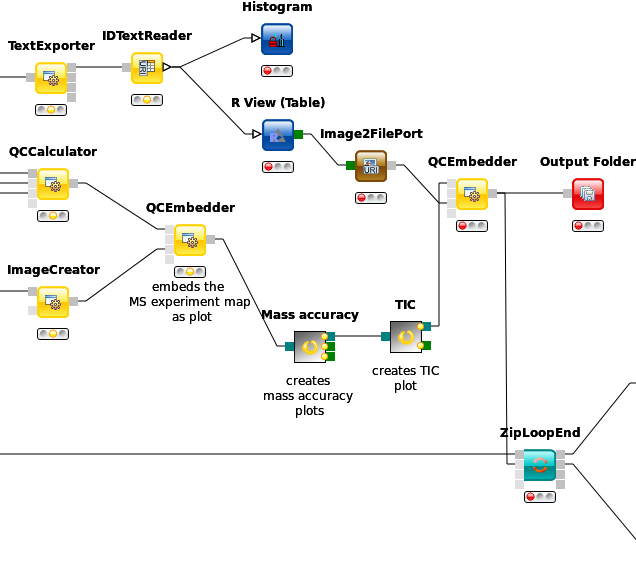
\includegraphics[width=0.65\textwidth]{graphics/qc/qc_extra}
  \caption{QC with new metric}
  \label{fig:qc_extra}
\end{figure}

\subsection{Set QC metrics}
\label{Set QC metrics}

Besides monitoring the quality of each individual mass spectrometry run analysis, another capability of QC with OpenMS and qcML is to monitor the complete set. The easiest control is to compare mass spectrometry runs which should be similar, e.g. technical replicates, to spot any aberrations in the set.\\
For this, we will first collect all created qcML files, merge them together and use the qcML onboard \textit{set QC} properties to detect any outliers.

\begin{itemize}
\item connect the \KNIMENODE{QCEmbedder}s output from last section to the \KNIMENODE{ZipLoopEnd}s second input port. 
\item The corresponding output port will collect all qcML files from each \KNIMENODE{ZipLoop} iteration and pass them on as a list of files.
\item Now we add a \KNIMENODE{QCMerger} node after the \KNIMENODE{ZipLoopEnd} and feed it that list of qcML files. In addition, we set its parameter \textit{setname} to give our newly created set a name - say \textit{spikein\_replicates}.
\item To now inspect all the QCs next to each other in that created qcML file, we have to add a new \KNIMENODE{Output Folder} to which we can connect the \KNIMENODE{QCMerger} output.
\end{itemize}
\newpage
When inspecting the set qcML file in a browser, we will be presented another overview. After the set content listing, the basic QC parameters (like number of identifications) are each displayed in a graph. Each set member (or run) has its own section on the x-axis and each run is connected with that graph via a link in the mouseover on one of the QC parameter values.


\begin{figure}[htbp]
  \centering
  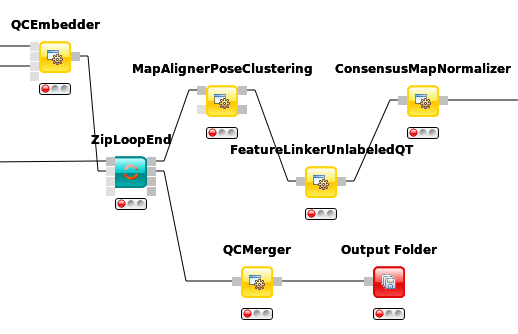
\includegraphics[width=0.85\textwidth]{graphics/qc/qc_set}
  \caption{QC set creation from ZipLoop}
  \label{fig:qc_set}
\end{figure}

\vspace{4cm}
\note{For ideas on new QC metrics and parameters -as you add them in your qcML files as generic parameters, feel free to contact us, so we can include them in the CV.}

